% !TEX root =  podc-submission.tex

\section{Proof of Correctness}

Consider any finite execution.  We must show that the linearization ordering $L$ defined in Section \ref{linearization} includes all operations that terminate and that 
(1) if an operation $op_1$ terminates before another operation $op_2$ begins, then $op_2$ cannot appear
before $op_1$ in $L$, and (2) each dequeue that terminates returns the same response as it would 
in $L$.

\here{need to update this outline later}
First, we define and prove some facts about blocks and the node's \nf{head} field. Then, we introduce  the linearization ordering formally. Next, we prove double \nf{Refresh} on a node is enough to propagate its children's new operations up to the node, which is used to prove (1). After this, we prove some claims about the size and operations of each block, which we use to prove the correctness of \nf{DoublingSearch()}, \nf{GetEnqueue()} and \nf{IndexDequeue()}. Finally, we prove the correctness of the way we compute the response of a dequeue, which establishes (2).

\subsection{Basic Properties}

A \typ{Block} object's fields, except for \fld{super}, are immutable:  they are written only 
when the block is created at line \ref{enqNew} or \ref{deqNew} (for a leaf's block) or lines \ref{initNewBlock}--\ref{computeLength} (for an internal node's block).  
Moreover, only a \op{CAS} at line \ref{setSuper1} can modify the \fld{super} field 
(from \nl\ to a non-\nl\ value), so it remains fixed once a value is stored in it.
Similarly, only a \op{CAS} at line \ref{cas} can modify an element of a node's \fld{blocks} array 
(from \nl\ to a non-\nl\ value), so once a block is stored in a node, it remains there forever.
Only a \op{CAS} at line \ref{incrementHead} can update a node's \head\ field by incrementing it,
which implies the following.

\begin{observation} \label{nonDecreasingHead}
For each node \var{v},  \var{v}.\fld{head} is non-decreasing over time.
\end{observation}

\begin{lemma} \label{lem::headInc}
Let $R$ be an instance of \opa{Refresh}{v} whose call to \op{CreateBlock} returns a non-\nl\ block.  When $R$ terminates, \var{v}.\head\ is greater than the value $R$ reads from it at line \ref{readHead}.
\end{lemma}
\begin{proof}
After $R$'s \op{CAS} at line \ref{incrementHead}, \var{v}.\head\ is no longer equal to the value \var{h}
read at line \ref{readHead}.  The claim follows from \Cref{nonDecreasingHead}.
\end{proof}

Now we show $v.\fld{blocks}[v.\head]$ is either the last non-\nl\ block or the first \nl\ block in node $v$.

\begin{invariant}\label{lem::headPosition} 
For $0 \leq i < v.\head$, $v.\fld{blocks}[i]\neq\nl$.  For $i>v.\head$, $v.\fld{blocks}[i]=\nl$.
\end{invariant}

\begin{proof}
Initially, $v.\head=1$, $v.\fld{blocks}[0]\neq\nl$  and $v.\fld{blocks}[i]=\nl$ for  $i>0$, so the claim~holds.

Assume the claim holds before a change to $v.\fld{blocks}$, which can be made only
by a successful \op{CAS} at line \ref{cas}.
The \op{CAS} changes $v.\fld{blocks}[h]$ from \nl\ to a non-\nl\ value.
Since $v.\fld{blocks}[h]$ is \nl\ before the CAS, $v.\head \leq h$ by the hypothesis.
Since $h$ was read from $v.\fld{blocks}[h]$ earlier at line \ref{readHead}, 
$v.\head \geq h$ by \Cref{lem::headPosition}.
So, $h=v.\head$ and a change to $v.\fld{blocks}[v.\head]$ preserves the invariant.

Now, assume the claim holds before a change to $v.\head$, which can only be an increment from $h$ to $h+1$
by a successful \op{CAS} at line \ref{incrementHead} of \op{Advance}.
It suffices to show that $v.\fld{blocks}[head] \neq \nl$.
\nf{Advance} is called either at line \ref{helpAdvance} 
after testing that $v.\fld{blocks}[h]\neq\nl$ at line \ref{ifHeadnotNull},
or at line \ref{advance} after the \op{CAS} at line \ref{cas} ensures $v.\fld{blocks}[h]\neq\nl$. 
\end{proof}

It follows that blocks accessed by the \op{Enqueue}, \op{Dequeue} and \op{CreateBlock} routines are non-\nl.

The following two lemmas show that no operation appears in more than one block of the root.
\begin{lemma} \label{lem::headProgress}
 If $b>0$ and $v.\fld{blocks}[b] \neq \nl$ then 
 $v.\fld{blocks}[b-1].\fld{end\sub{left}} \leq v.\fld{blocks}[b].\fld{end\sub{left}}$ and 
 $v.\fld{blocks}[b-1].\fld{end\sub{right}} \leq v.\fld{blocks}[b].\fld{end\sub{right}}$.
\end{lemma}
\begin{proof}
Let $B$ be the block in $v.\fld{blocks}[b]$.
Before creating $B$ at line \ref{invokeCreateBlock}, the \op{Refresh} that installed $B$
read $b$ from $v.\head$ at line \ref{readHead}.
At that time, $v.\fld{blocks}[b-1]$ contained a block $B'$, by \Cref{lem::headPosition}.
Thus, the \op{CreateBlock}($v,b-1$) that created $B'$ terminated before the \op{CreateBlock}($v,b$) that
created $B$ started.
It follows from \Cref{nonDecreasingHead} that the value that 
line \ref{createEndLeft} of \op{CreateBlock}($v,b-1$) stores in $B'.\fld{end\sub{left}}$   
is less than or equal to the value that line \ref{createEndLeft} of \op{CreateBlock}($v,b$) 
stores in $B.\fld{end\sub{left}}$.
Similarly, the values stored in $B'.\eright$ and $B.\eright$ at line \ref{createEndRight} 
%of these calls to \op{CreateBlock} 
satisfy the claim.
\end{proof}

\begin{lemma} \label{lem::subblocksDistinct}
If $B$ and $B'$ are two blocks in nodes at the same depth, their sets of subblocks are disjoint.
\end{lemma}
\begin{proof}
We prove the lemma by reverse induction.
If $B$ and $B'$ are in leaves, they have no subblocks, so the claim is true.
Assume the claim is true for nodes at depth $d+1$ and let $B$ and $B'$ be two blocks in nodes at depth $d$.
Consider the direct subblocks of $B$ and $B'$ defined by (\ref{defsubblock}).
If $B$ and $B'$ are in different nodes at depth $d$, then their direct subblocks are disjoint.
If $B$ and $B'$ are in the same node, it follows from \Cref{lem::headProgress} that their direct subblocks are disjoint.
Either way, their direct subblocks (at depth $d+1$) are disjoint, so the claim follows from the induction hypothesis.
\end{proof}

It follows that each block has at most one superblock.
Moreover, we can now prove each operation is contained in at most one block of each node,
and hence appears at most once in the linearization~$L$.

\begin{corollary}\label{lem::noDuplicates}
For  $i\neq j$, $v.\fld{blocks}[i]$ and $v.\fld{blocks}[j]$ cannot both contain the same operation.
\end{corollary}
\begin{proof}
The operations contained in a block $B$ are those that appear in subblocks of $B$ in the leaves of the tree.
Since each process puts each of its operations in only one block of its own leaf, an operation 
cannot be in two different leaf blocks. 
By \Cref{lem::subblocksDistinct}, $v.\fld{blocks}[i]$ and $v.\fld{blocks}[j]$ have no subblocks in common, so the claim follows.
\end{proof}



%\begin{definition}
%$n\nf{.blocks[}i\nf{]}$ is \emph{established} if $n\nf{.head}>i$. An operation is \it{established} in node $n$ 
%if it is in an established block of $n$. $EST^t_n$ is the set of established operations in node $n$ at time $t$.
%\end{definition}
%
%Now we want to say that blocks of a node grow over time.
%\begin{observation}\label{lem::blocksOrder}
%  If  time $t<$ time $t^\prime$ ($t$ is before $t^\prime$), then $ops(n.blocks)$ at time $t$ is a subset of 
%$ops(n.blocks)$ at time $t^\prime$.
%\end{observation}
%\begin{proof}
%Blocks are only appended (not modified) with \nf{CAS} to $n\nf{.blocks[}n\nf{.head]}$, so the set of the blocks of a node after the \nf{CAS} contains the set of the blocks before the \nf{CAS}.
%\end{proof}

% \begin{corollary}\label{lem::establishedOrder}
%   If  time $t<$ time $t^\prime$, then $EST_n^t\subseteq EST_n^{t^\prime}$.
% \end{corollary}
% \begin{proof}
% From Observations \ref{nonDecreasingHead}, \ref{lem::blocksOrder}.  
% \end{proof}

The following shows that the values stored in \fld{sum\sub{enq}} and \fld{sum\sub{deq}} fields are accurate.
\here{If space is tight, could easily move next proof to appendix and just say it follows easily from the definition of subblocks and the values stored in the fields on lines \ref{enqNew}, \ref{deqNew}, \ref{createSumEnq}, \ref{createSumDeq}.}

\begin{invariant}\label{lem::sum}
If $B$ is a block stored in $v.\fld{blocks}[i]$,
$B.\fld{sum\sub{enq}} = | E(v.\fld{blocks}[0])\cdots E(v.\fld{blocks}[i]) |$ and
$B.\fld{sum\sub{deq}} = | D(v.\fld{blocks}[0])\cdots D(v.\fld{blocks}[i]) |$.
\end{invariant}
\begin{proof}
Initially, each \fld{blocks} array only contains an empty block $B_0$ in location 0.
By definition, $E(B_0)$ and $D(B_0)$ are empty sequences.
Moreover, $B_0.\fld{sum\sub{enq}} = B_0.\fld{sum\sub{deq}} = 0$, so the claim is true.

We show that each installation of a block $B$ into some location $v.\fld{blocks}[i]$ preserves the claim,
assuming the claim holds before this installation.  We consider two cases.

If $v$ is a leaf, $B$ was created at line \ref{enqNew} or \ref{deqNew}.
For line \ref{enqNew}, $B$ represents a single enqueue operation, so $|E(B)|=1$ and $|D(B)|=0$.
Moreover, $B.\fld{sum\sub{enq}}$ is set to $v.\fld{blocks}[i-1]+1$ and
$B.\fld{sum\sub{deq}}$ is set to $v.\fld{blocks}[i-1]$, so the claim follows from the hypothesis.
The proof for line \ref{deqNew}, where $B$ represents a single dequeue operation is similar.

Now suppose $v$ is an internal node. By the definition of subblocks in (\ref{defsubblock}), the
subblocks of $v.\fld{blocks}[1..i]$ are $v.\fld{left.blocks}[1..B.\eleft]$ 
and $v.\fld{right.blocks}[1..B.\eright]$.
Thus, the enqueues in $E(v.\fld{blocks}[0])\cdots E(v.\fld{blocks}[i])$ are those in
$E(v.\fld{left.blocks}[0]) \cdots E(v.\fld{left.blocks}[B.\eleft])$ and
$E(v.\fld{left.blocks}[0]) \cdots E(v.\fld{left.blocks}[B.\eright])$.
By the hypothesis, the total number of these enqueues is $v.\fld{left.blocks}[B.\eleft].\fld{sum\sub{enq}} + v.\fld{right.blocks}[B.\eright].\fld{sum\sub{enq}}$, which is the value that line \ref{createSumEnq} stored in $B.\fld{sum\sub{enq}}$ when $B$ was created.
The proof for \fld{sum\sub{deq}} (stored on line~\ref{createSumDeq}) is similar.
\end{proof}

This allows us to prove that every block a Refresh installs contains at least one operation.

\begin{corollary}\label{blockNotEmpty}
If a block $B$ is in $v.\fld{blocks}[i]$ where $i>0$, then $E(B)$ and $D(B)$ are not both empty.
\end{corollary}
\begin{proof}
The \op{Refresh} that installed $B$ got $B$ as the response to its call to \op{CreateBlock} on line \ref{invokeCreateBlock}.
Thus, at line \ref{testEmpty} $\var{num\sub{enq}}+\var{num\sub{deq}}\neq 0$.
By \Cref{lem::sum}, $\var{num\sub{enq}} = |E(B)|$ and $\var{num\sub{deq}} = |D(B)|$,
so these sequences cannot both be empty.
\end{proof}



\subsection{Propagating Operations to the Root}
Next, we show two \op{Refresh}es suffice to propagate operations from a child to its parent.
We say that node $v$ \emph{contains} an operation if some block in $v.\fld{blocks}$ contains the operation.
\here{move this defn earlier and just recall it here?}
Once a block is added to a node, it remains there forever.  Thus, if $v$ contains an operation at some time, it contains the operation at all later times too.

\begin{lemma}\label{successfulRefresh}
Let $R$ be a call to \op{Refresh}($v$) that performs a successful \op{CAS} on line \ref{cas} (or terminates at line \ref{addOP}).
In the configuration after that CAS (or termination, respectively), $v$ contains all operations that $v$'s children contained 
when $R$ executed line~\ref{readHead}.
\end{lemma}
\begin{proof}
Suppose $v$'s child (without loss of generality, $v.\fld{left}$) contained an operation $op$ 
in the configuration $C$ immediately before $R$ executed line \ref{readHead}.
Then some block $B$ in $v.\fld{left.blocks}[i]$ contains $op$.
By \Cref{nonDecreasingHead} and \Cref{lem::headProgress}, the value of $childHead$ that $R$ reads from
$v.\fld{left.head}$ in line \ref{readChildHead} is at least $i$.
If it is equal to $i$, $R$ calls \op{Advance} at line \ref{helpAdvance}, which ensures that 
$v.\fld{left.head} > i$.
Then, $R$ calls \op{CreateBlock}($v,h$) in line \ref{invokeCreateBlock}, where $h$ is the value $R$ reads at line \ref{readHead}.
\op{CreateBlock} reads a value greater than $i$ from $v.\fld{left.head}$ at line \ref{createEndLeft}.
Thus, $new.\eleft \geq i$.  We consider two cases.

Suppose $R$'s call to \op{CreateBlock} returns the new block $B'$ and $R$'s \op{CAS} at line \ref{cas} 
installs $B'$ in $v.\fld{blocks}$.
Then, $B$ is a subblock of some block in $v$, since  $B'.\eleft$ is greater than or equal to $B$'s index
in $v.\fld{left.blocks}$.
Hence $B'$ contains $op$, as required.

\Eric{I think this case was missing from the proof in the thesis}
Now suppose $R$'s call to \op{CreateBlock} returns \nl, causing $R$ to terminate at line \ref{addOP}.
Intuitively, since there are no operations in $v$'s children to promote, $op$ is already in $v$.
We formalize this intuition.
The value computed at line \ref{createSumEnq} is
\begin{eqnarray*}
\var{num\sub{enq}} 
&=& v.\fld{left.blocks}[new.\eleft].\fld{sum\sub{enq}} + v.\fld{right.blocks}[new.\eright].\fld{sum\sub{enq}} - v.\fld{blocks}[h-1].\fld{sum\sub{enq}} \\
&=& v.\fld{left.blocks}[new.\eleft].\fld{sum\sub{enq}} + v.\fld{right.blocks}[new.\eright].\fld{sum\sub{enq}} \\
&&\mbox{ }- v.\fld{left.blocks}[v.\fld{blocks}[h-1].\eleft].\fld{sum\sub{enq}} - v.\fld{right.blocks}[v.\fld{blocks}[h-1].\eright].\fld{sum\sub{enq}}
\end{eqnarray*}
It follows from \Cref{lem::sum} that $num\sub{enq}$ is the total number of enqueues contained in the blocks
$v.\fld{left.blocks}[v.\fld{blocks}[h-1].\eleft+1..new.\eleft]$ and
$v.\fld{right.blocks}[v.\fld{blocks}[h-1].\eright+1..new.\eright]$.
Similarly, $num\sub{deq}$ is the total number of dequeues contained in these blocks.
Since $num\sub{enq}+num\sub{deq}=0$ at line \ref{testEmpty},
these blocks contain no operations.
By \Cref{blockNotEmpty}, this means the ranges of blocks are empty, so that $v.\fld{blocks}[h-1].\eleft \geq new.\eleft \geq i$.
Hence, $B$ is already a subblock of some block in $v$, so $v$ contains $op$.
\end{proof}

We now show that if a process fails its \op{Refresh}($v$) twice, some other process must have succeeded.

\begin{lemma}\label{lem::doubleRefresh}
Consider two consecutive terminating calls $R_1$, $R_2$ to \nf{Refresh}($v$) by the same process.
When $R_2$ terminates, $v$ contains all operations that $v$'s children contained when $R_1$ was invoked.
\end{lemma}
\begin{proof}
If either $R_1$ or $R_2$ performs a successful \op{CAS} at line \ref{cas} or terminates at line \ref{addOP}, the claim follows
from Lemma \ref{successfulRefresh}.
So suppose both $R_1$ and $R_2$ perform a failed \op{CAS} at line \ref{cas}.
Let $h_1$ and $h_2$ be the values $R_1$ and $R_2$ read from $v.\head$ at line \ref{readHead}.
By \Cref{lem::headInc}, $h_2>h_1$.
By \Cref{lem::headProgress}, $v.blocks[h_2]=\nl$ when $R_1$ executes line \ref{readHead}.
Since $R_2$ fails its \op{CAS} on $v.blocks[h_2]$, some other \op{Refresh} $R_3$ must have done
a successful \op{CAS} on $v.blocks[h_2]$ before $R_2$'s \op{CAS}.
$R_3$ must have executed line \ref{readHead} after $R_1$, since $R_3$ read the value $h_2$ from $v.\head$ and the value of $v.\head$ is non-decreasing, by \Cref{nonDecreasingHead}.
Thus, all operations contained in $v$'s children when $R_1$ begins
are also contained in $v$'s children when $R_3$ later executes line \ref{readHead}.
By \Cref{successfulRefresh}, these operations are contained in $v$ when $R_3$ performs its successful \op{CAS},
which is before $R_2$ terminates.
\end{proof}

\begin{lemma} \label{lem::appendExactlyOnce}
When an \op{Append}($B$) terminates, $B$'s operation is contained in exactly one block in each node along the path from the process's leaf to the root.
\end{lemma}
\begin{proof}
The \op{Append} adds $B$ to the process's leaf and calls \op{Propagate}, which
performs a double \op{Refresh} on each node along the path from the leaf's parent to the root.
By \Cref{lem::doubleRefresh}, this ensures $B$'s operation is contained in each node along this path.
By \Cref{lem::noDuplicates}, it is contained in exactly one block in each node.
\end{proof}

\subsection{Correctness of GetEnqueue}
-------


\nf{DoublingSearch($e$, $end$)} returns a pair \nf{<$b$, $i$>} such that the $i$th \nf{Enqueue} in the $b$th block of the root is the $e$th \nf{Enqueue} in the sequence stored in the root. 

\begin{lemma}[\nf{DoublingSearch} correctness]\label{dsearch}
If $1\leq e \leq \nf{root.blocks[$end$].sum\sub{enq}}$, then \nf{Doubling-}\\\nf{Search($e$, $end$)} returns \nf{<$b$, $i$>} such that $E_i(root,b)= E_e(root)$.
\end{lemma}
\begin{proof}
 From Lines \ref{setSumEnqLeft} and \ref{setSumEnqRight} we know the \nf{sum\sub{enq-left}}, and \nf{sum\sub{enq-right}} fields of \nf{blocks} in each node are sorted in non-decreasing order. Since $\nf{sum\sub{enq}}=\nf{sum\sub{enq-left}}+ \nf{sum\sub{enq-right}}$, the $\nf{sum\sub{enq}}$ values of \nf{root.blocks[$0\cdot\cdot end$]} are also non-decreasing. By Corollary~\ref{lem::sumX} we know that the \nf{sum\sub{enq}} field in a block is the sum of the number of \nf{Enqueue} operations in that block and the all blocks before that block in the node. Furthermore, since $\nf{root.blocks[$0$].sum\sub{enq}}=0$ and $\nf{root.blocks[$end$].sum\sub{enq}} \geq e$, there is a $b$ such that $\nf{root.blocks[$b-1$].sum\sub{enq}}<e$ and $e\leq\nf{root.blocks[$b$].sum\sub{enq}}$. Block \nf{root.blocks[$b$]} contains $E_i(root,b)$.  Lines \ref{dsearchStart}--\ref{dsearchEnd} doubles the search range in Line \ref{doubling} and will eventually reach \nf{start} such that $\nf{root.blocks[start].sum\sub{enq}}\leq e \leq\nf{root.blocks[end].sum\sub{enq}}$. Then, in Line \ref{dsearchBinarySearch}, the binary search finds the $b$ such that \nf{root.blo- cks[$b-1$].sum\sub{enq}$<e\leq$root.blocks[$b$].sum\sub{enq}}. By Corollary \ref{lem::sumX}, \nf{root.blocks[$b$]} is the block that contains $E_e(root)$. Finally, $i$ is computed using the definition of \nf{sum\sub{enq}} and Corollary \ref{lem::sumX}.
\end{proof}

\begin{lemma}[\nf{GetEnqueue} correctness] \label{get}
If $1\leq i \leq \nf{$n$.blocks[$b$].num\sub{enq}}$ then \nf{$n$.GetEnqueue($b$, $i$)} returns $E_i(n,b)$\nf{.element}.
\end{lemma}
\begin{proof}
We will prove this lemma by induction on the node $n$'s height. For the base case, suppose $n$ is a leaf. Leaf blocks each contain exactly one operation, $n\nf{.blocks[$b$].sum\sub{enq}}\leq 1$, which means only \nf{$n$.GetEnqueue(b,1)} can be called when $n$ is a leaf and $n$\nf{.blocks[$b$]} must contain an \nf{Enqueue} operation. Line \ref{getBaseCase} of \nf{$n$.GetEnqueue($b$, $1$)} returns the \nf{element} of the \nf{Enqueue} operation stored in the $b$th block of leaf ${n}$, as required.

For the induction step, we prove if \nf{$n$.dir.GetEnqueue($b^\prime$, $i$)} returns $E_i(n.\nf{dir}, b^\prime)$ then \nf{$n$.GetE-}\\\nf{nqueue($b$,~$i$)} returns $E_i(n,b)$.  From Definition \ref{ordering} of $E(n,b)$, we know that operations from the left subblocks come before the operations from the right subblocks in a block (see Figure \ref{figGet}). By Lemma \ref{lem::numX}, the \nf{num\sub{enq-left}} field  in \nf{$n$.blocks[$b$]} is the number of \nf{Enqueue} operations from the blocks' subblocks in the left child of $n$. So the $i$th \nf{Enqueue} operation in $n\nf{.blocks[}b\nf{]}$ is propagated from the right child if and only if $i$ is greater than $n\nf{.blocks[}b\nf{]}$\nf{.num\sub{enq-left}}. Line \ref{leftOrRight} decides whether the $i$th enqueue in the $b$th block  of internal node $n$ is in the  left child or right child subblocks of \nf{$n$.blocks[$b$]}. By Definitions \ref{def::subblock} and \ref{def::ops}, to find an operation in the subblocks of \nf{$n$.blocks[$b$]} we need to search in the range
\begin{align*}
&\texttt{$n$.left.blocks[$n$.blocks[$b$-1].end\textsubscript{left}+1..$n$.blocks[$b$].end\textsubscript{left}]}  \textrm{ or } \\
&\texttt{$n$.right.blocks[$n$.blocks[$b$-1].end\textsubscript{right}+1..$n$.blocks[$b$].end\textsubscript{right}]}.
 \end{align*}
First, we consider the case where the \nf{Enqueue} we are looking for is in the left child. There are $eb=n.\nf{blocks[}b-1\nf{].sum\sub{enq-left}}$ \nf{Enqueue}s in the blocks of $n$\nf{.left} before the left subblocks of $n$\nf{.blocks[$b$]}, so $E_i(n,b)$ is $E_{i+eb}(n.\tt{left})$ which is $E_{i^\prime}(n.\tt{left},b^\prime)$ for some $b^\prime$ and $i^\prime$. We can compute $b^\prime$ and then search for the $i^\prime$th \nf{Enqueue} in \tt{$n$.left.blocks[$b^\prime$]}, where $i^\prime$ is $i+eb-n$\tt{.left.blocks[}$b^\prime-1$\tt{].sum\sub{enq}}. The parameters in Line~\ref{leftChildGet} are for searching $E_{i+eb}(n\nf{.left})$ in \nf{$n$.left.blocks} in the range of left subblocks of $n$\nf{.blocks[}$b$\nf{]}, so this \nf{BinarySearch} returns the index of the subblock containing $E_i(n,b)$.

Otherwise, the \nf{Enqueue} we are looking for is in the right child. Because \nf{Enqueue}s from the left subblocks are ordered before the ones from the right subblocks, there are \nf{n.blocks[b].num\sub{enq-left}} enqueues ahead of $E_i(n,b)$ from the left child. So we need to search for $i-n\nf{.blocks[}b\nf{].num\sub{enq-left}}+ n\nf{.blocks[}b-1\nf{].sum\sub{enq-right}}$ in the right child (Line \ref{rightChildGet}). Other parameters for the right child are chosen similarly to the left child. 

So, in both cases, the direct subblock containing $E_i(n,b)$ is computed in Line \ref{leftChildGet} or \ref{rightChildGet}.
$subblockIndex$ is the index of the block in $n.\nf{dir}$ containing $E_i(n,b)$. Finally, \nf{$n$.child.GetEnqueue( $subblockIndex$, $i$)} is invoked  and it returns $E_i(n,b)$\nf{.element} by the hypothesis of the induction.
\end{proof}

\begin{figure}[hbt]  
  \center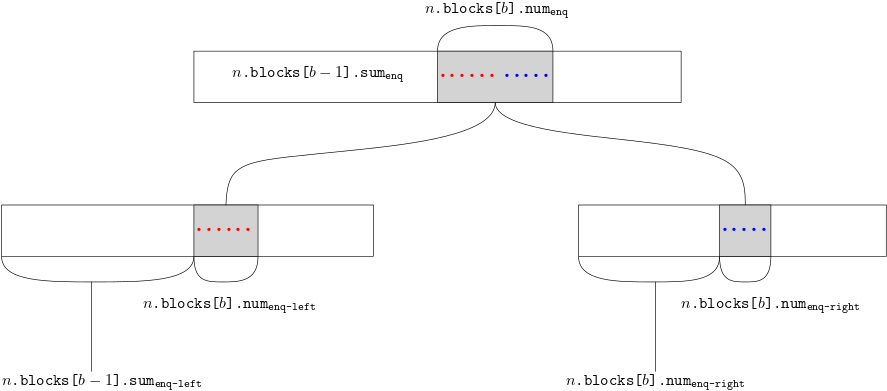
\includegraphics[width=6in]{pics/blockSumEnq.png}
  
  \caption[\nf{Enqueue} operations propagated from the left and the right child to a node.]{The number and order of the \nf{Enqueue} operations propagated from the left and the right child to \nf{$n$.blocks[$b$]}. Both \nf{$n$.blocks[$b$]} and its subblocks are shown in grey. \nf{Enqueue} operations from the left child (colored red), are ordered before the \nf{Enqueue} operations from the right child (colored blue).
  }\label{figGet}
\end{figure}


\subsection{Correctness of IndexDequeue}
The next few results show that the \nf{super} field of a block is accurate within one of the actual index of the block's superblock in the parent node. 
\here{mention that precondition of IndexDequeue follows; also check that block of parent indexed by sup in that routine is non-null}
Then we explain how it is used to compute the rank of a given \nf{Dequeue} in the root.
\begin{definition}\label{orderRefresh} If a \nf{Refresh} instance $R_1$ does its \nf{CAS} at Line \ref{cas} earlier than \nf{Refresh} instance $R_2$ we say $R_1$ has \it{happened before} $R_2$.
\end{definition}

\begin{observation} \label{setSupBeforeIncHead}
After \nf{$n$.blocks[$i$].CAS(null, $B$)} succeeds, \nf{$n$.head} cannot increase from ${i}$ to ${i+1}$ until \nf{$B$.super} is set.
\end{observation}
\begin{proof}
From Observation \ref{nonDecreasingHead} we know that \nf{$n$.head} changes only by the increment on Line \ref{incrementHead}. Before an instance of \nf{Advance} increments \nf{n.head} on Line \ref{incrementHead}, Line \ref{setSuper1} ensures that \nf{n.blocks[head].super} was set at Line \ref{setSuper1}.
\end{proof}

\begin{corollary}
  If \nf{$n$.blocks[$i$].super} is \nf{null}, then $\nf{$n$.head}\leq i$ and \nf{$n$.blocks[$i+1$]} is \nf{null}.
\end{corollary}
\begin{proof}
By Invariant \ref{lem::headPosition} and Observation \ref{setSupBeforeIncHead}.
\end{proof}
Now let us consider how the \nf{Refresh}es that took place on the parent of node $n$ after block $B$ was stored in $n$ will help to set \nf{$B$.super} and propagate $B$ to the parent.

\begin{observation}\label{lem::createBlockHead}
If the block created by an instance $R_p$ of $n$\nf{.parent.Refresh} contains block $B=n$\nf{.blocks[}$b$\nf{]} then $R_p$ reads a value greater than $b$ from $n$\nf{.head} in Line \ref{lastLine}. 
\end{observation}

\begin{lemma}
  If $B=n$\nf{.blocks[}$b$\nf{]} is a direct subblock of \nf{$n$.parent.blocks[$superblock$]} then $\nf{$B$.super}\leq superblock$.
\end{lemma}
\begin{proof}
Let $R_p$ be the instance of $n$\nf{.parent.Refresh} that does a successful \nf{CAS}(Line~\ref{cas}) and puts the superblock of $B$ which is $n$\nf{.parent.blocks[$superblock$]} into $n\nf{.parent}$. By Observation~\ref{lem::createBlockHead} if $R_p$ propagates $B$ it has to read a greater value than $b$ from \nf{$n$.head}, which means \nf{$n$.head} was incremented from $b$ to $b+1$ in Line \ref{incrementHead}. By Observation \ref{setSupBeforeIncHead} \nf{$B$.super} was already set in Line \ref{setSuper1}. The value written in \nf{$B$.super}, was read in Line \ref{readParentHead} before the \nf{CAS} that sets \nf{$B$.super} in Line \ref{setSuper1}. From Observation \ref{nonDecreasingHead} we know \nf{$n$.parent.head} is non-decreasing so $B\nf{.super}\leq superblock$, since \nf{$n$.parent.head} is still equal to $superblock$ when $R_p$ executes its \nf{CAS} at Line \ref{cas} by Lemma \ref{lem::headProgress}. The reader may wonder when the case $b\nf{.super}=superblock$ happens. This can happen when $\nf{$n$.parent.blocks[$B$.super]}=\nf{null}$ when $B$\nf{.super} is written and $R_p$ puts its created block into \nf{$n$.parent.blocks[$B$\nf{.super}]} afterwards.
\end{proof}

\begin{lemma}\label{lem::secondRefreshSuper}
Let $R_n$ be a \nf{Refresh} that puts $B$ in \nf{$n$.blocks[$b$]} at Line \ref{cas}. Then, the block created by one of the next two successful \nf{$n$.parent.Refresh}es according to Definition \ref{orderRefresh} contains $B$ and \nf{$B$.super} is set when the second successful \nf{$n$.parent.Refresh} reaches Line \ref{invokeCreateBlock}.
\end{lemma}

\begin{proof}
Let $R_{p1}$ and $R_{p2}$ be the next two successful \nf{$n$.parent.Refresh}es after $R_n$. To derive a contradiction assume $B$ was neither propagated to $n$\nf{.parent} by $R_{p1}$ nor by $R_{p2}$.

Since $R_{p2}$'s created block does not contain $B$, by Observation \ref{lem::createBlockHead} the value $R_{p2}$ reads from $n$\nf{.head} in Line \ref{lastLine} is at most $b$. From Observation \ref{nonDecreasingHead} the value $R_{p2}$ reads in Line \ref{readChildHead} is also at most~$b$.

$R_n$ puts $B$ into $n$\nf{.blocks[}$b$\nf{]} so ${R_n}$ reads the value $b$ from $n.$\nf{head}. Since $R_{p2}$'s \nf{CAS} into $n$\nf{.parent.blocks} is successful there should be a \nf{Refresh} instance $R_p^\prime$ on $n$\nf{.parent} that increments $n$\nf{.parent.head} (Line \ref{incrementHead}) after $R_{p1}$'s Line \ref{cas} and before $R_{p2}$'s Line \ref{readHead}. We assumed $t^{R_n}_{\ref{cas}}<t^{R_{p1}}_{\ref{cas}}<t^{R_{p2}}_{\ref{cas}}$ by Definition \ref{orderRefresh}. Finally, Line \ref{readChildHead} is after Line \ref{readHead} and $R_{p2}$'s Line \ref{readHead} is after $R_p^\prime$'s Line \ref{incrementHead}, which is after ${R_n}$'s $n$\nf{.blocks.CAS}. 
\begin{align*}
\left.
\begin{array}{r}
 _{\ref{cas}}^{R_n}t<_{\ref{cas}}^{R_{p1}}t\\
_{\ref{cas}}^{R_{p1}}t<_{\ref{incrementHead}}^{R_{p^\prime}}t<_{\ref{readHead}}^{R_{p2}}t\\
_{\ref{readHead}}^{R_{p2}}t<_{\ref{readChildHead}}^{R_{p2}}t\\
\end{array}
\right\} &\Longrightarrow  _{\ref{cas}}^{R_n}t<_{\ref{readChildHead}}^{R_{p2}}t
\end{align*}

So $R_{p2}$ reads a value greater than or equal to $b$ for $n.\nf{head}$ by Observation \ref{nonDecreasingHead}.

Therefore $R_{p2}$ reads $n\nf{.head}=b$. $R_{p2}$ calls $n$\nf{.Advance} at Line \ref{helpAdvance}, which ensures $n$\nf{.head} is incremented from $b$. So the value $R_{p2}$ reads in Line \ref{lastLine} of \nf{CreateBlock} is greater than $b$ and $R_{p2}$'s created block contains $B$. This is in contradiction with our hypothesis.

Furthermore, if $B$\nf{.super} was not set earlier, it is set by $R_{p2}$'s call to $n$\nf{.Advance} invoked from Line~\ref{helpAdvance}.
\end{proof}

\begin{corollary} \label{superRelation}
If \nf{$B=n$.blocks[$b$]} is propagated to $n$\nf{.parent}, then \nf{$B$.super} is equal to or one less than the index of the superblock of $B$.
\end{corollary}
\begin{proof}
% After that $B$ is installed, $n$\nf{.parent.head} is read, and $B.$\nf{super} field is set to the value read from the parent's \nf{head} (see Lines \ref{readParentHead} and \ref{setSuper1} of\nf{Advance}).
Let $R_n$ be the \nf{$n$.Refresh} that put $B$ in $n$\nf{.blocks} and let $R_{p1}$ be the first successful \nf{$n$.parent.Refresh} after $R_n$ and $R_{p2}$ be the second next successful \nf{$n$.parent.Refresh}.
Before $B$ can be propagated to $n$'s \nf{parent}, $n$\nf{.head}  must be greater than $b$, so by Observation \ref{setSupBeforeIncHead} $B$\nf{.super} is set.
From Lemma \ref{lem::secondRefreshSuper} we know that $B$ is propagated by the second next successful \nf{Refresh}'s \nf{CAS} on $n$\nf{.parent.blocks}. To summarize, we have $n\nf{.parent.head}_{_{\ref{cas}}^{R_{p2}}t}= n\nf{.parent.head}_{_{\ref{cas}}^{R_{p1}}t}+1$ and  $n\nf{.parent.head}_{_{\ref{cas}}^{R_{p1}}t}\leq n\nf{.parent.head}_{_{\ref{cas}}^{R_n}t}$ from Definition \ref{orderRefresh} and Observation \ref{nonDecreasingHead}. The value that is set in $B$\nf{.super} is read from $n$\nf{.parent.head} after ${_{\ref{cas}}^{R_n}t}$. So $B$\nf{.super} is equal to or one less than the index of the superblock of $B$.
\end{proof}

We prove \nf{IndexDequeue}'s correctness using Corollary \ref{superRelation} on each step of the \nf{IndexDequeue}.

\begin{lemma}[\nf{IndexDequeue} correctness]
 If $1\leq i \leq\nf{$n$.blocks[$b$].num\sub{deq}}$ then \nf{$n$.IndexDequeue($b$,$i$)} returns $<x,y>$ such that $D_i(n,b)=D_y(\nf{root},x)$.
\end{lemma}
\begin{proof}
We will prove this by induction on the distance of $n$ from the \nf{root}. The base case where $n$ is \nf{root} is trivial (see Line \ref{indexBaseCase}).
For the non-root nodes \nf{$n$.IndexDequeue($b$, $i$)} computes $superblockIndex$, the index of the superblock of the $b$th block in $n$, in Line \ref{computeSuper} by Corollary \ref{superRelation}. After that, the position of $D_i(n,b)$ in $D(n.\nf{parent}, superblockIndex)$ is computed in Lines \ref{computeISuperStart}--\ref{computeISuperEnd}. By Definition \ref{ordering}, \nf{Dequeue}s in a block are ordered based on the order of its subblocks  from left to right. If $D_i(n,b)$ was propagated from the left child, the number of dequeues in the left subblocks of \nf{$n$.parent.blocks[$superblockIndex$]} before \nf{$n$.blocks[$b$]} is considered in Line \ref{considerPreviousLeft} (see Figure \ref{fig::blockSumDeqLeft}). Otherwise, if $D_i(n,b)$ was propagated from the right child, the number of dequeues in the subblocks from the left child is considered to be ahead of the computed index (Line \ref{considerRight}) (see Figure \ref{fig::blockSumDeqRight}). Finally, \nf{IndexDequeue} is called on \nf{$n$.parent} recursively, and it returns the correct response by the induction hypothesis. 
\end{proof}
\begin{figure}[hbt]  
  \center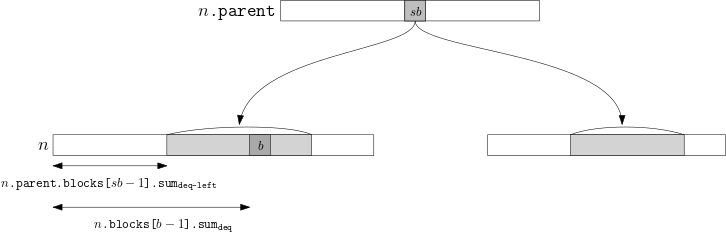
\includegraphics[width=6in]{pics/blockSumDeqLeft.png}
  
  \caption[Number of \nf{Dequeue} operations before a \nf{Dequeue} in a left child.]{The number of \nf{Dequeue} operations before $D_i(n,b)$ shown in the case where $n$ is a left child. The index of the superblock is shown with $sb$. }\label{fig::blockSumDeqLeft}
\end{figure}
\begin{figure}[hbt]  
  \center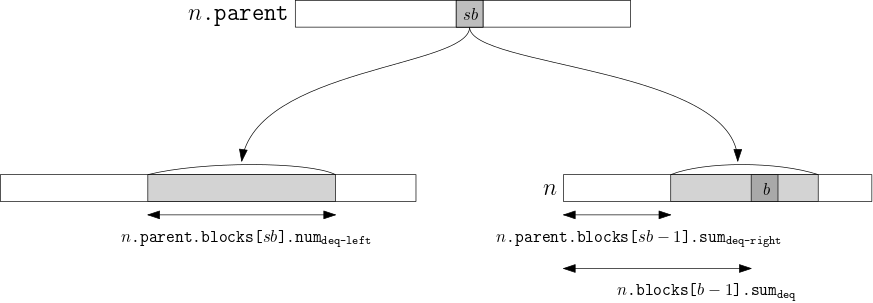
\includegraphics[width=6in]{pics/blockSumDeqRight.png}
  
  \caption[Number of \nf{Dequeue} operations before a \nf{Dequeue} in a right child.]{The number of \nf{Dequeue} operations before $D_i(n,b)$ shown in the case where $n$ is a right child. The index of the superblock is shown with $sb$. }\label{fig::blockSumDeqRight}
\end{figure}

\subsection{Linearizability}
We now prove the two properties needed for linearizability.

\begin{lemma} \label{linearSat}
$L$ is a legal linearization ordering.
\end{lemma}
\begin{proof}
We must show for any execution that every operation that terminates is in $L$ exactly once. Also, if $op_{1}$ terminates before $op_{2}$ in starts in the execution, then $op_{1}$ is before $op_{2}$ in the linearization. The first claim is directly reasoned from Corollary \ref{lem::appendExactlyOnce}. For the latter, if $op_{1}$ terminates before $op_{2}$ starts,  $op_{1}$\nf{.Append} has terminated before $op_{2}$\nf{.Append} started. From Corollary \ref{lem::append}, $op_{1}$ is in \nf{root.blocks} before $op_{2}$ starts to propagate. By definition of $L$, $op_{1}$ is linearized before $op_{2}$.
\end{proof}
Once some operations are aggregated in one block, they will get propagated up to the root together, and they can be linearized in any order among themselves. We have chosen to put \nf{Enqueue}s in a block before \nf{Dequeue}s (see Definition \ref{ordering}).

\begin{definition}\label{defNullDeq}
If a \nf{Dequeue} operation returns \nf{null} it is called a \it{null} \nf{Dequeue}, otherwise it is called \it{non-null}~\nf{Dequeue}.
\end{definition}

Next, we define the responses that \nf{Dequeue}s should return, according to the linearization.
\begin{definition}
   Assume the operations in \nf{root.blocks} are applied sequentially on an empty queue in the order of $L$.  ${Resp(d)=e}$\nf{.element} if the element of \nf{Enqueue} $e$ is the response to \nf{Dequeue} $d$. Otherwise if ${d}$ is a null \nf{Dequeue} then ${Resp(d)=\nf{null}}$. 
\end{definition}

In the next lemma, we show that the \nf{size} field in each \nf{root block} is computed correctly.
\begin{lemma}\label{sizeCorrectness}
  \nf{root.blocks[$b$].\size}is the \size of the queue after the operations in \nf{root.blocks[$0 \cdot$\\$\cdot\cdot b$]} are applied in the order of~$L$.  
\end{lemma}
\begin{proof}
We prove the claim by induction on $b$. The base case when ${b=0}$ is trivial since the queue is initially empty and $\nf{root.blocks[}0\nf{]}$ contains an empty block with \nf{size} field equal to $0$. We are going to show the correctness when $b=i$ assuming  correctness when $b=i-1$. By Definition \ref{ordering} \nf{Enqueue} operations come before \nf{Dequeue} operations in a block in $L$. By Lemma~\ref{lem::numX} \nf{num\sub{enq}} and \nf{num\sub{deq}} fields in a block show the number of \nf{Enqueue} and \nf{Dequeue} operations in it. If there are more than $\nf{root.blocks[}i-1\nf{].size}+\nf{root.blocks[}i\nf{].num\sub{enq}}$ dequeue operations in \nf{root.blocks[$i$]} then the queue would become empty after \nf{root.blocks[$i$]}. Otherwise, the size of the queue after the $b$th block in the root is $\nf{root.blocks[}b-1\nf{].size}+ \nf{root.blocks[}b\nf{].num\sub{enq}}- \nf{root.blocks[}b\nf{].num\sub{deq}}$. In both cases, this is the same as the assignment on Line \ref{computeLength}.
\end{proof}

The next lemma is useful to compute the number of non-null dequeues.
\begin{lemma} \label{numberOfNND}
If operations in the root are applied in the order of $L$, the number of non-null \nf{Dequeue}s in $\nf{root.blocks[}0\cdots b\nf{]}$ is \nf{root.blocks[$b$].sum\sub{enq} $-$ root.blocks[$b$].size}.
\end{lemma}
\begin{proof}
There are \nf{root.blocks[$b$]}\nf{.sum\sub{enq}} \nf{Enqueue} operations in $\nf{root.blocks[}0\cdots b\nf{]}$ by Corollary~\ref{lem::sumX}. The size of the queue after doing $\nf{root.blocks[}0\cdots b\nf{]}$ in the order of $L$ is 
the number of $\it{enqueues}$ in $\nf{root.blocks[}0\cdots b\nf{]}$ minus the number of $\it{non-null \nf{Dequeue}s}$ in $\nf{root.blocks[}0\cdots b\nf{]}$. By the correctness of the \nf{size} field from Lemma \ref{sizeCorrectness} and \nf{sum\sub{enq}} field from Lemma \ref{lem::numX}, the number of $\it{non-null \nf{Dequeue}s}$ is \nf{root.blocks[$b$]}\nf{.sum\sub{enq}} $-$ \nf{root.blocks[$b$]}\nf{.size}. 
\end{proof}

\begin{corollary}\label{numNullDeqBlock}
  If operations in the root are applied in the order of $L$, the number of non-null dequeues in $\nf{root.blocks[}b\nf{]}$ is \nf{root.blocks[$b$].num\sub{enq} $-$ root.blocks[$b$].\size $+$ root.blocks[$b-1$].size}.
\end{corollary}

\begin{lemma}\label{nullReturn}
$Resp(D_i(\nf{root},b))$ is \nf{null} iff \nf{root.blocks[$b-1$].\size $+$ root.blocks[$b$].num\sub{enq}$- i$ $<0$}.
\end{lemma}
\begin{proof}
The claim follows immediately from Corollary  \ref{numNullDeqBlock} and Lemma \ref{lem::numX}.
\end{proof}

\begin{lemma}\label{computeHead}
\nf{FindResponse($b$, $i$)} returns $Resp(D_i(root,b))$.
\end{lemma}
\begin{proof}
$D_i(root,b)$ is $D_{\nf{root.blocks[}b-1\nf{].sum\sub{deq}}+i}(root)$ by Definition \ref{ordering} and Lemma \ref{lem::sumX}. $D_i(root,b)$ returns \nf{null} at Line \ref{returnNull} if $\nf{root.blocks[}b-1\nf{].size}+ \nf{root.blocks[}b\nf{].num\sub{enq}}- i <0$ and $Resp(D_i(root,b))=\nf{null}$ in this case by Lemma \ref{nullReturn}. Otherwise, if $D_i(root,b)$ is the $e$th non-null \nf{Dequeue} in $L$ it should return the $e$th enqueued value. By Lemma \ref{numberOfNND} there are \nf{root.blocks[$b-1$].sum\sub{enq} $-$ root.blocks[$b-1$].\size} non-null \nf{Dequeue} operations in $\nf{root.blocks[}0\cdots b-1\nf{]}$. The \nf{Dequeue}s in \nf{root.blocks[$b$]} before $D_i(root,b)$ are non-null \nf{Dequeue}s. So $D_i(root,b)$ is the $e$th non-null \nf{Dequeue} where $e= i + \nf{root.blocks[}b-1\nf{].sum\sub{deq}} - \nf{root.blocks[}b-1\nf{].size}$ (Line \ref{computeE}). See Figure \ref{computeResponseDetail}.

After computing $e$ at Line \ref{computeE}, the code finds \nf{$b$,$i$} such that $E_i(root,b)=E_e(root)$ using \nf{DoublingSearch} and then finds its \nf{element} using \nf{GetEnqueue} (Line \ref{findAnswer}). Correctness of \nf{DoublingS-}\\\nf{earch} and \nf{GetEnqueue} routines are shown in Lemmas \ref{dsearch} and \ref{get}.
\end{proof}

\begin{figure}[hbt]  
  \center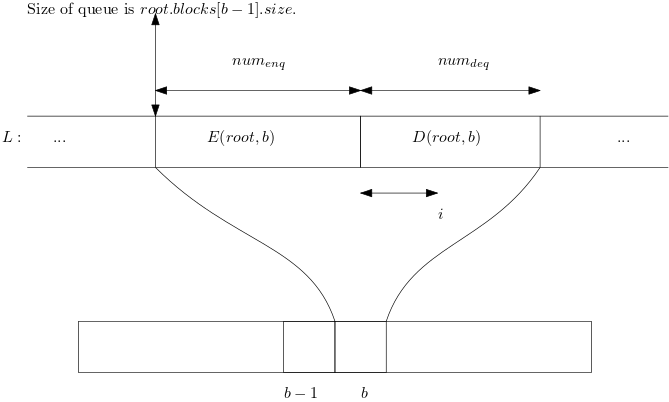
\includegraphics[width=4in, height=2.5in]{pics/computeResponseDetail.png}\caption{The position of $D_i(root,b)$.}
\label{computeResponseDetail}
\end{figure}
\vspace{-1em}

\begin{lemma}\label{linearCorrect}
The responses to operations in our algorithm are the same as in the sequential execution in the order given by $L$.
\end{lemma}
\begin{proof}
\nf{Enqueue} operations do not return any value. By Lemma \ref{computeHead}, the response of a \nf{Dequeue} in our algorithm is the same as its response in the sequential execution of $L$.  
\end{proof}

\begin{theorem}[Main]
The queue implementation is linearizable.
\end{theorem}
\begin{proof}
The theorem follows from Lemmas \ref{linearSat} and \ref{linearCorrect}.
\end{proof}

\paragraph{Remark} In fact our algorithm is strongly linearizable as defined in \cite{DBLP:conf/stoc/GolabHW11}. By Definition \ref{ordering} the linearization ordering of operations will not change as blocks containing new operations are appended to the root.


\here{following material from algorithm description in thesis might be useful in sketch of correctness proof}
\begin{figure}[hbpt]
  \center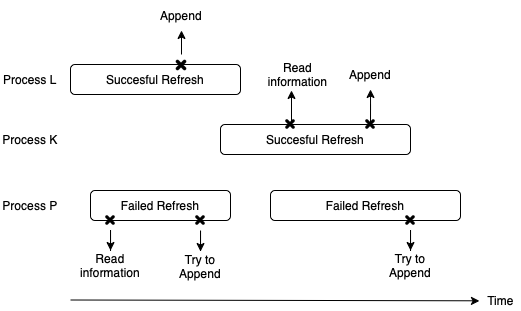
\includegraphics[width=4in]{pics/doublyrefresh-drawio.png}
  \caption[Two consecutive failed \nf{Refresh}es by a
    process.]{\label{fig::simpleDoubleRefresh}Time relations between
    the concurrent successful \nf{Refresh}es and the two consecutive
    failed \nf{Refresh}es.} 
\end{figure}
We use \nf{CAS} (Compare\&Swap) instructions to implement the
\nf{Refresh}'s attempt to append  described in the previous
paragraph. 
The second failed \nf{Refresh} of $P$ is assuredly concurrent with a
successful \texttt{Refresh} that has read its information after the
invocation of the first failed \nf{Refresh} (see Figure
\ref{fig::simpleDoubleRefresh}). This is because some process $L$ does
a successful append during $P$'s first failed attempt, and some
process $K$ performs a \nf{Refresh} that reads its information after
$L$'s append and then performs a successful append during $P$'s second
failed \nf{Refresh}. Process $K$'s \nf{Refresh} helps to append the
new operations that were in $n$'s children before $P$'s first failed
\nf{Refresh}, in case they were not already appended. After a process
appends its operation into its leaf it can call \nf{Refresh} on the
path up to the root at most two times on each node. So, with $O(\log
p)$ \nf{CAS}es an operation can ensure it appears in the
linearization. This cooperative solution allows us to overcome the CAS
Retry Problem. 


